\subsection{Helioviewer}\label{ssec:hv}

SunPy provides the ability to download images from Helioviewer Project
servers.  The aim of the Helioviewer Project is to enable the
exploration of solar and heliospheric data from multiple data sources
(such as instrumentation and feature/event catalogs) via easy-to-use
visual interfaces.  The primary data provided by the Helioviewer
Project are images in the JPEG2000 format (for further details on the
Helioviewer Project see \cite{}\footnote{SunPy is used in Helioviewer
  production servers to manage the download and ingestion of JPEG2000
  files from remote servers.}.)

In

Suppose we next want to download a PNG image of the latest AIA 304
image available on Helioviewer.org. We could use the explicit
approach:

\begin{listing}
\begin{minted}{python}
hv.download_png('2099/01/01', 4.8, "[SDO,AIA,AIA,304,1,100]", x0=0, y0=0, width=512, height=512)
\end{minted}
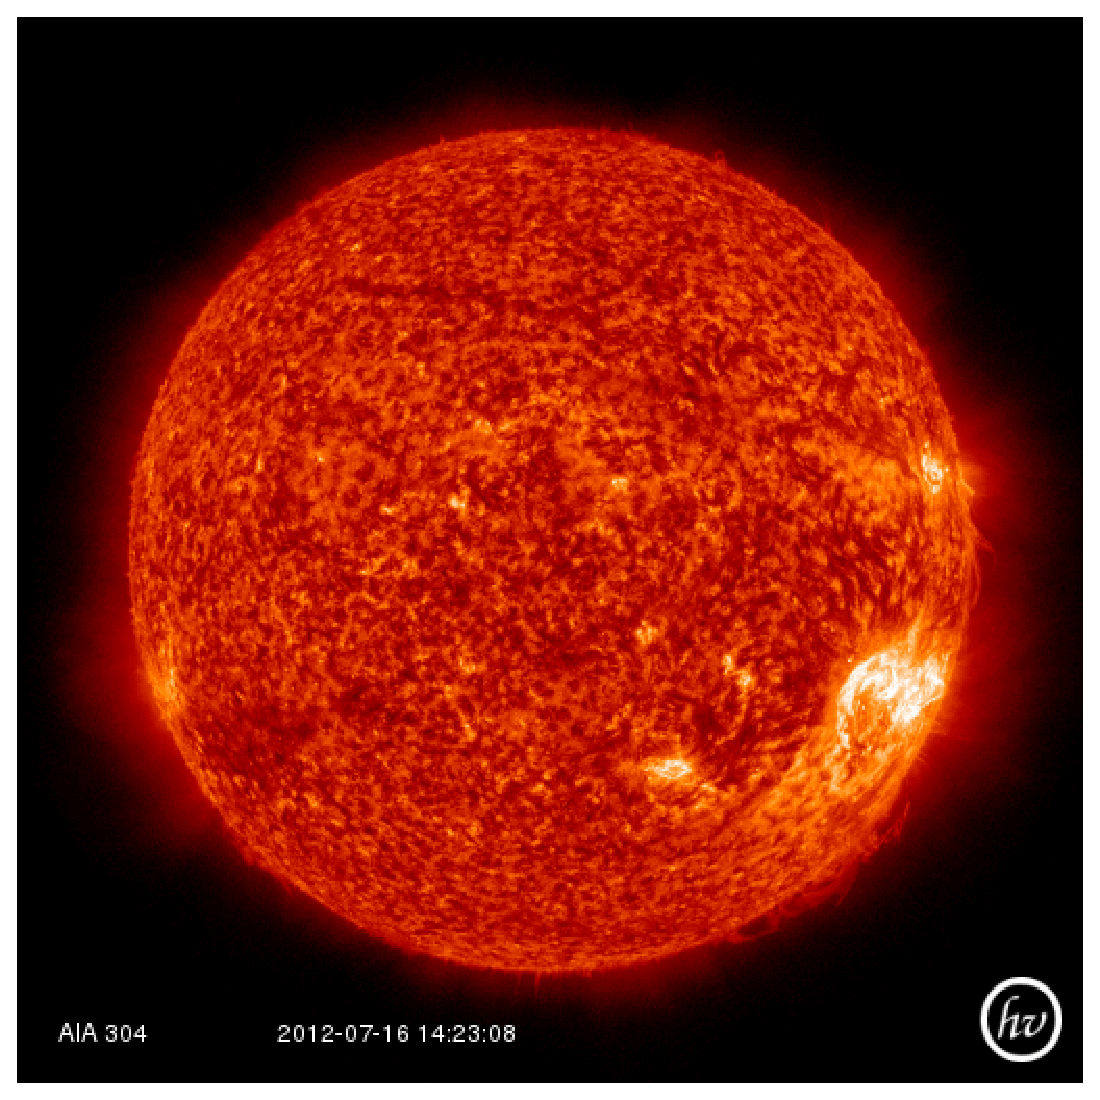
\includegraphics[width=0.8\columnwidth]{helioviewer_latest_aia_304.eps}
\caption{Acquisition of a PNG file showing the latest AIA 304\AA\ image available at
  www.helioviewer.org.}
\label{code:downloadlatestpng}
\end{listing}

Where 4.8 refers to the image resolution in arcseconds per pixel
(larger values mean lower resolution), the “1” and “100” in the layer
string refer to the visibility (visible/hidden) and opacity, x0 and y0
are the center points about which to focus and the width and height
are the pixel values for the image dimensions.


The filename of the returned file has the date and time of the
requested time, which is not the time of the observation shown in the
PNG image.  This is because of the Helioviewer API.  The API request
finds images closest to the requested time. But since the user may ask
for images from multiple sources, and each of them may have a
different observation time, it is unclear which time is the most
appropriate to associate with the resultant image.  The Helioviewer
API does not select between any of the image observation times, but
instead returns an image filename based on the request time, resulting
in predictable filenames.

The Helioviewer API allows composition and overlay of images from
multiple sources, based on the positioning metadata in the source FITS
file. This ability takes advantage of the fact that the JPEG2000 file
format contains an arbitrary XML box that can be used to store image
metadata.  Helioviewer Project JPEG2000 file metadata are based (in
part) on the original FITS header information, and carry sufficient
metadata to permit overlay with other Helioviewer JPEG2000 files.

SunPy accesses this overlay/composition capability through the
\texttt{download_png} method of the Helioviewer client.

\begin{listing}
\begin{minted}{python}
hv.download_png('2099/01/01', 6, "[SDO,AIA,AIA,304,1,100],[SDO,AIA,AIA,193,1,50],[SOHO,LASCO,C2,white-light,1,100]", x0=0, y0=0, width=768, height=768)
\end{minted}
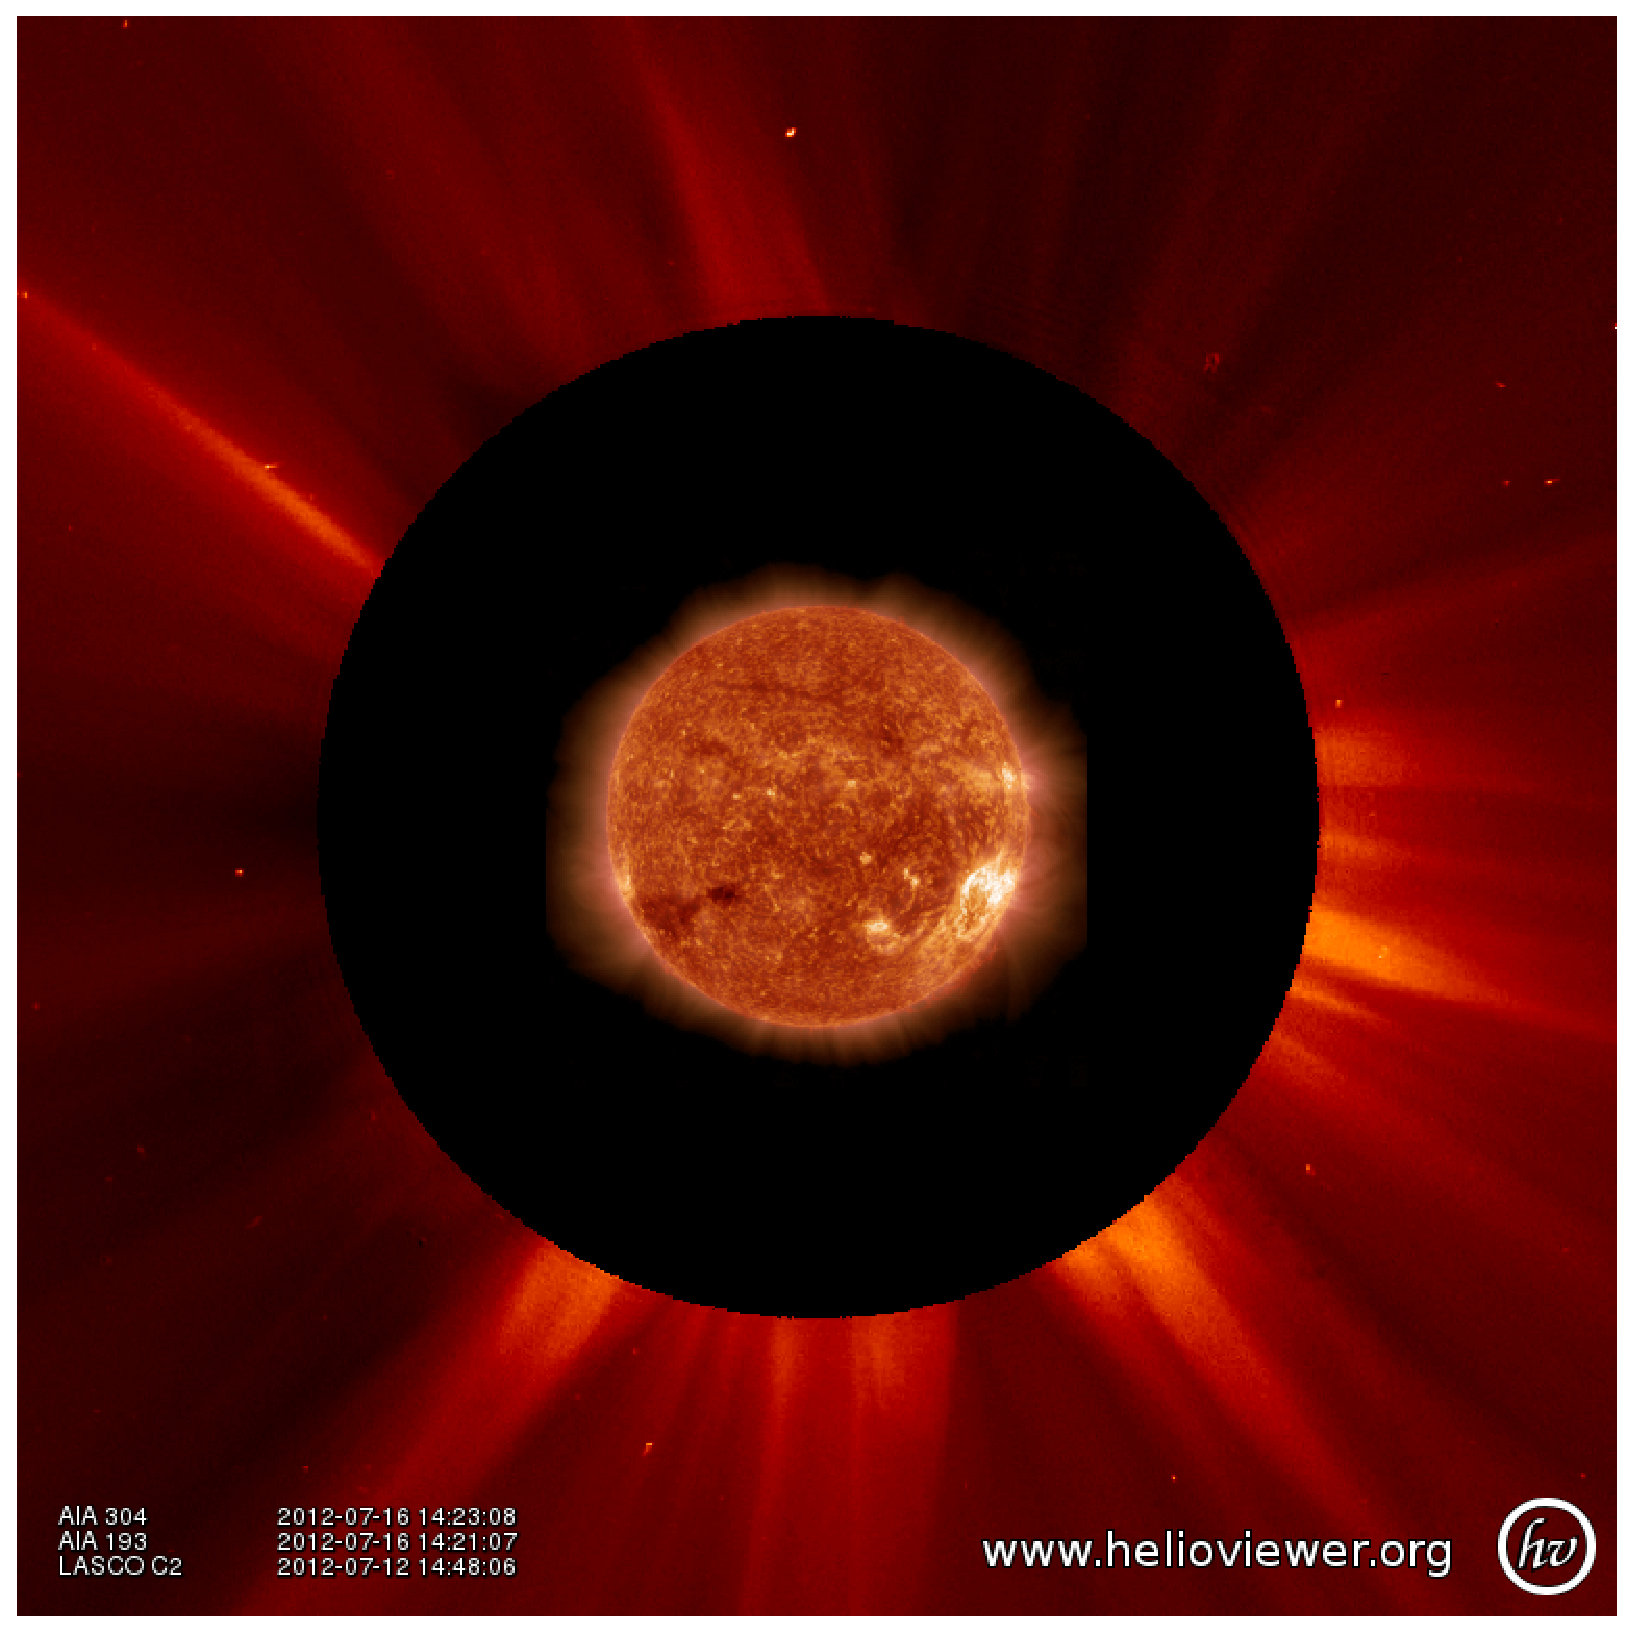
\includegraphics[width=0.8\columnwidth]{helioviewer_overlay_example.eps}
\caption{Acquisition of a PNG image composed from data from three
  separate sources.}
\label{code:downloadjp2}
\end{listing}

This functionality makes it simple for SunPy users to generate complex
images from multiple, correctly overlaid, image datasources. 



To read a JPEG2000 file into a SunPy session requires installing two
other pieces of software. The first, \texttt{OpenJPEG}, is an open
source library for reading and writing JPEG2000 files
(http://www.openjpeg.org).  The other package required is
\texttt{glymur}, (https://github.com/quintusdias/glymur), an interface
between Python and the OpenJPEG libraries (note that these packages
are {\it not} required to use the functionality described above).


Listing \ref{code:downloadjp2} demonstrates the querying, reading and
conversion of a Helioviewer JPEG2000 file into a SunPy Map object.
This functionality allows users to visualize and manipulate
Helioviewer-supplied image data in an identical fashion to a SunPy map
object generated from FITS data (see Section \ref{sec:maps}).

\begin{listing}
\begin{minted}{python}
filepath = hv.download_jp2('2012/07/05 00:30:00', observatory='SDO', instrument='HMI', detector='HMI', measurement='continuum')
from sunpy.map import Map
hmi = Map(filepath)
hmi.submap([200,550],[-400,-200]).peek()
\end{minted}
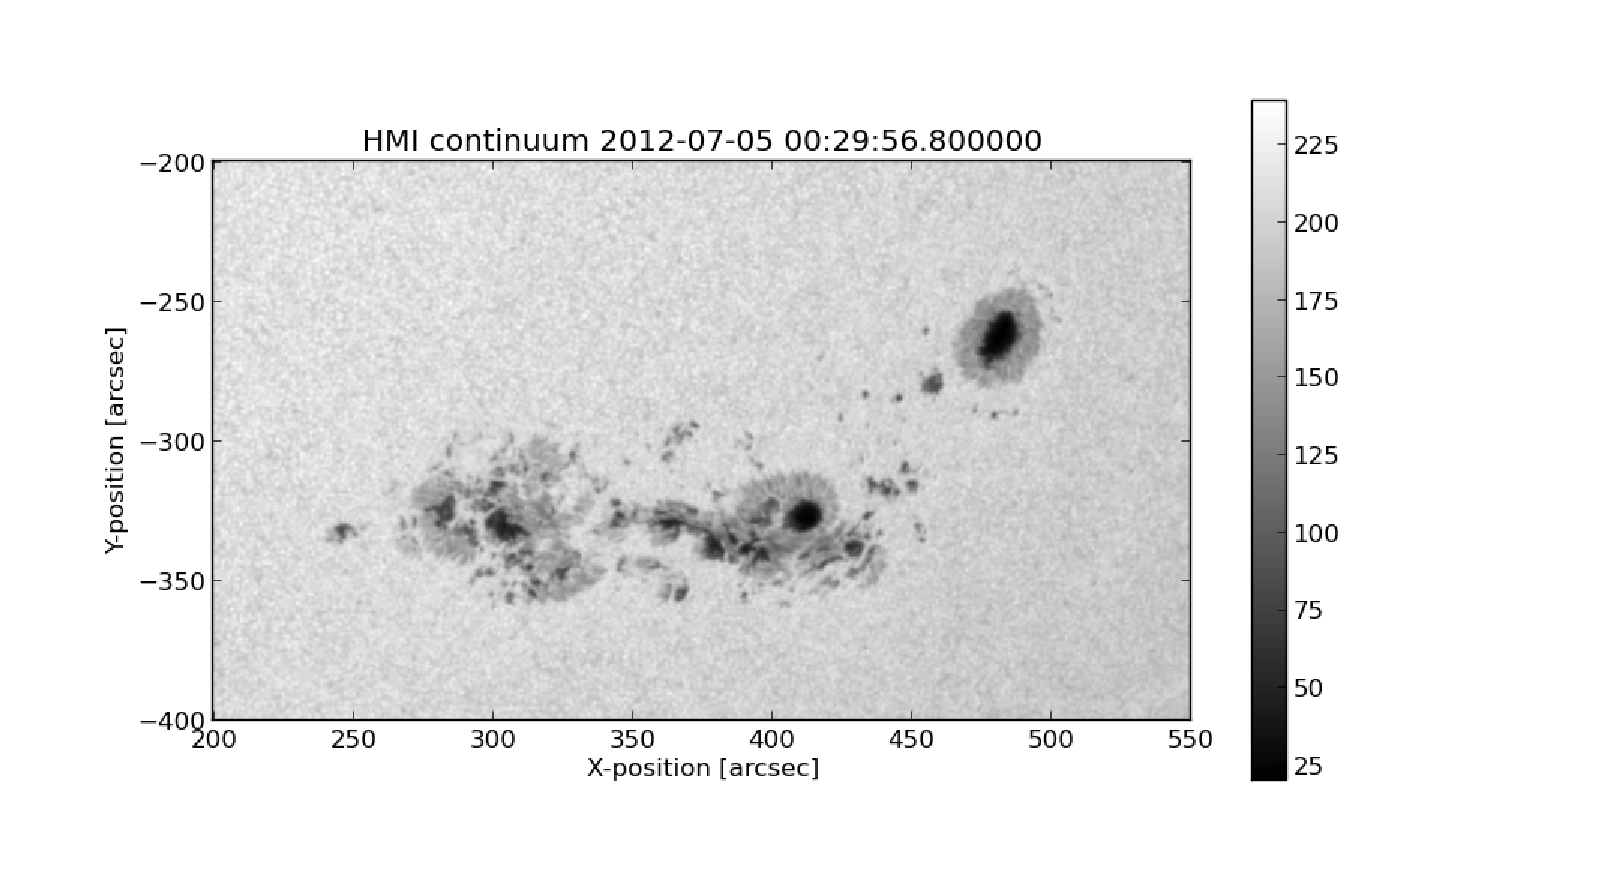
\includegraphics[width=0.8\columnwidth]{helioviewer_hmi_continuum_jp2_to_map.eps}
\caption{Acquisition and display of a Helioviewer JPEG2000 file as a
  SunPy map object.}
\label{code:downloadjp2}
\end{listing}


